%% The Incomparable's Skeletor Clip Loop Chart
%% http://alexwlchan.net/skeletor/
%%
%% This chart tracks the progess of Steve Lutz's attempt to create
%% a recursive clip loop in the annual clip show going all the way
%% back to the Skeletor clip.
%%
%% To build this file, you'll need:
%%
%%  * XeLaTeX with the hyperref, fontspec, xcolor and tikz packages
%%    (all of which are included with most standard LaTeX distros)
%%  * The Patua One and Oxygen fonts (freely downloadable from Google)
%%
%% Then compile the file as `xelatex skeletor.tex`.

\documentclass{standalone}

\usepackage{hyperref}
\usepackage{fontspec}
\usepackage{tikz}

\usepackage{xcolor}
\definecolor{incompblue}{HTML}{242B6F}

\setsansfont{Patua One}
\setmainfont{Oxygen}
\setmonofont{Oxygen}  % for URLs

\renewcommand{\baselinestretch}{1.15}

\newcommand*{\episode}[3]{
  \fill [incompblue] (#1) circle (0.4);
  \draw (#1) node (#1title) [below=20pt, align=center, text width=6cm]
    {\large{\textbf{#2}}};
  \draw (#1title.south) node [below=4pt, align=center, text width=6cm] {#3};
}

\newcommand*{\link}{
  \draw [->, incompblue, line width=3pt, shorten >=0.45cm]
}

\let\origurl=\url
\renewcommand*{\url}[1]{\textcolor{incompblue}{\origurl{#1}}}

\def\hspacing{6.8cm}

\makeatletter
\newcommand{\HUGE}{\@setfontsize\Huge{38}{47}}
\makeatother

\begin{document}
  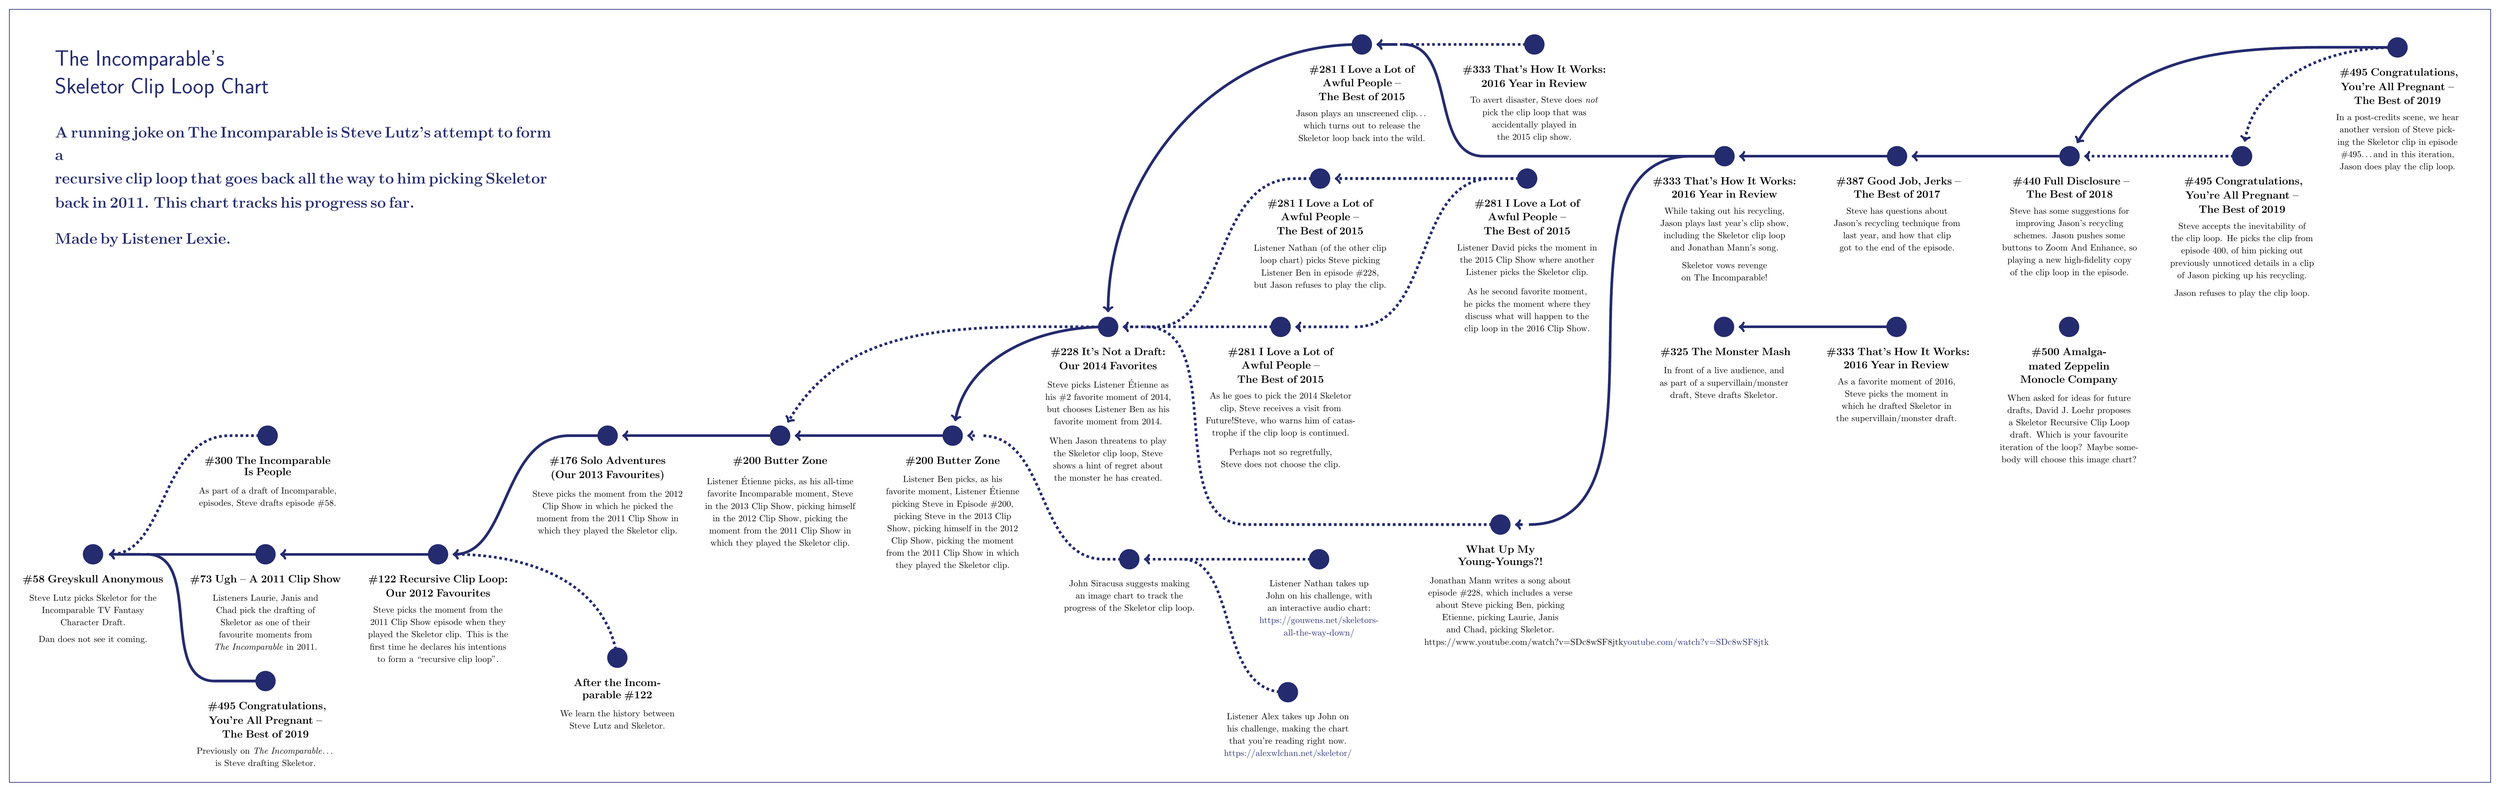
\begin{tikzpicture}

    \draw [incompblue, thick] (-3.3, -9) rectangle (94.5, 21.5);

    \draw [incompblue] (8.5, 16) node [align=left, text width=20cm] (title) {\textsf{\HUGE{%
      The\, Incomparable's \\[8pt] %
      Skeletor\, Clip\, Loop\, Chart}} \\[24pt]
      {\textbf{\LARGE{%
        A running joke on The Incomparable is Steve Lutz's attempt to form a \\[1pt] %
        recursive clip loop that goes back all the way to him picking
        Skeletor \\[2pt] %
        back in 2011.  This chart tracks his progress so far. \\[24pt]
        Made by Listener Lexie.
      }}}
    };

    \coordinate (ep58) at (0, 0);
    \episode{ep58}{\#58 Greyskull Anonymous}{%
      Steve Lutz picks Skeletor for the \\%
      Incomparable TV Fantasy \\%
      Character Draft. \\[5pt] %
      Dan does not see it coming.
    }

    \draw (ep58) ++ (0:\hspacing) node (ep73) {};
    \episode{ep73}{\#73 Ugh -- A 2011 Clip Show}{%
      Listeners Laurie, Janis and \\
      Chad pick the drafting of \\
      Skeletor as one of their favourite moments from \\%
      \textit{The Incomparable} in 2011.%
    }
    \draw (ep58) ++ (0.05, 0) node (ep58r1) {};
    \link (ep73) -- (ep58r1);

    % https://www.theincomparable.com/theincomparable/495/
    \draw (ep58) ++ (0:\hspacing) ++ (0, -5) node (ep495_previously) {};
    \episode{ep495_previously}{
      \#495 Congratulations, You're All Pregnant -- \\[2pt]
      The Best of 2019
    }{
      Previously on \emph{The Incomparable}\ldots \\
      is Steve drafting Skeletor.
    }
    \draw (ep58) ++ (2, 0) node (ep58_right) {};
    \link (ep495_previously) -- ++ (-2, 0) to [out=180, in=0] (ep58_right) -- (ep58r1);

    \draw (ep73) ++ (0:\hspacing) node (ep122) {};
    \episode{ep122}{\#122 Recursive Clip Loop: \\[2pt] Our 2012 Favourites}{%
      Steve picks the moment from the %
      2011 Clip Show episode when they %
      played the Skeletor clip. This is the %
      first time he declares his intentions \\ %
      to form a ``recursive clip loop''.
    }
    \link (ep122) -- (ep73);

    \draw (ep122) ++ (-30:1.2*\hspacing) node (ep122b) {};
    \episode{ep122b}{After the Incomparable \#122}{%
      We learn the history between \\%
      Steve Lutz and Skeletor.%
    }
    \link [dashed] (ep122b) to [out=100, in=0] (ep122);

    \draw (ep122) ++ ( 35:1.2*\hspacing) node (ep176) {};
    \episode{ep176}{\#176 Solo Adventures \\[2pt] (Our 2013 Favourites)}{%
      Steve picks the moment from the %
      2012 Clip Show in which he picked %
      the moment from the 2011 Clip Show %
      in which they played the Skeletor clip.
    }
    \link (ep176) -- ++ (-1.5, 0) to [in=0, out=180] (ep122);

    \draw (ep176) ++ (0:\hspacing) node (ep200et) {};
    \episode{ep200et}{\#200 Butter Zone}{%
      Listener \'Etienne picks, as his %
      all-time favorite Incomparable moment, %
      Steve in the 2013 Clip Show, picking %
      himself in the 2012 Clip Show, picking %
      the moment from the 2011 Clip Show %
      in which they played the Skeletor clip.
    }
    \link (ep200et) -- (ep176);

    \draw (ep200et) ++ (0:\hspacing) node (ep200b) {};
    \episode{ep200b}{\#200 Butter Zone}{%
      Listener Ben picks, as his \\favorite moment, Listener \'Etienne %
      picking Steve in Episode \#200, %
      picking %
      Steve in the 2013 Clip Show, picking %
      himself in the 2012 Clip Show, picking %
      the moment from the 2011 Clip Show %
      in which they played the Skeletor clip.
    }
    \link (ep200b) -- (ep200et);

    \draw (ep200b) ++ (35:1.1*\hspacing) node (ep228) {};
    \episode{ep228}{\#228 It's Not a Draft: \\[2pt] Our 2014 Favorites}{%
      Steve picks Listener \'Etienne as his \#2 favorite moment of 2014, \\%
      but chooses Listener Ben as his favorite moment from 2014. \\[8pt]%
      When Jason threatens to play the %
      Skeletor clip loop, Steve shows %
      a hint of regret about the %
      monster he has created.
    }
    \link (ep228) to [out=180, in=80] (ep200b);
    \link [dashed] (ep228) to [out=180, in=60] (ep200et);

    \draw (ep200b) ++ (-35:1.25*\hspacing) node (siracusa) {};
    \episode{siracusa}{}{}
    \draw (siracusa) node [below=20pt, align=center, text width=6cm] {%
      John Siracusa suggests making \\ %
      an image chart to track the progress of the Skeletor clip loop.};
    \draw (ep200b) ++ (1, 0) node (ep200bright) {};
    \link [dashed] (siracusa) -- ++ (-1, 0) to [out=180, in=0] (ep200bright) -- (ep200b);

    \draw (siracusa) ++ (0:1.1 * \hspacing) node (nathan) {};
    \episode{nathan}{}{}
    \draw (nathan) node [below=20pt, align=center, text width=6cm] {%
      Listener Nathan takes up John on his challenge, with an interactive audio chart: \\%
      \url{https://gouwens.net/skeletors-all-the-way-down/}
    };
    \link [dashed] (nathan) -- (siracusa);

    \draw (siracusa) ++ (-40:1.2 * \hspacing) node (alex) {};
    \episode{alex}{}{}
    \draw (alex) node [below=20pt, align=center, text width=6cm] {%
      Listener Alex takes up John on his challenge, making the chart that you're reading right now.
      \url{https://alexwlchan.net/skeletor/}
    };
    \draw (siracusa) ++ (1.5, 0) node (sirright) {};
    \link [dashed, -] (alex) to [out=180, in=00, shorten >=1cm] (sirright);

    \draw (ep228) ++ (0:\hspacing) node (ep281) {};
    \episode{ep281}{%
      \#281 I Love a Lot of \\[-1pt] %
      Awful People --\\[2pt] %
      The Best of 2015}{%
      As he goes to pick the 2014 Skeletor %
      clip, Steve receives a visit from \\%
      Future!Steve, who %
      warns him of catastrophe %
      if the clip loop is continued. \\[8pt]
      Perhaps not so regretfully, Steve does not choose the clip.
    }
    \link [dashed] (ep281) -- (ep228);

    \draw (ep228) ++ (35: 1.5*\hspacing) node (ep281nathan) {};
    \episode{ep281nathan}{%
      \#281 I Love a Lot of \\[-1pt] %
      Awful People --\\[2pt] %
      The Best of 2015}{%
      Listener Nathan (of the other clip %
      loop chart) picks Steve picking \\ %
      Listener Ben in episode \#228, %
      but Jason refuses to play the clip.
    }
    \draw (ep228) ++ (1.3, 0) node (ep228right) {};
    \link [dashed, -] (ep281nathan) -- ++ (-1, 0) to [out=180, in=00] (ep228right);

    \draw (ep281nathan) ++ (0:1.2*\hspacing) node (ep281david) {};
    \episode{ep281david}{%
      \#281 I Love a Lot of \\[-1pt] %
      Awful People --\\[2pt] %
      The Best of 2015}{%
      Listener David picks the moment in the 2015 Clip Show where another Listener picks the Skeletor clip. \\[8pt]
      As he second favorite moment, he picks the moment where they discuss what will happen to the clip loop in the 2016 Clip Show.
    }
    \link [dashed] (ep281david) -- (ep281nathan);
    \draw (ep281) ++ (2.8, 0) node (ep281right) {};
    \link [dashed] (ep281david) ++ (-1.4, 0) to [out=180, in=0] (ep281right) -- (ep281);

    \draw (ep228) ++ (55:2*\hspacing) ++ (2.2, 0) node (ep281clip) {};
    \episode{ep281clip}{%
      \#281 I Love a Lot of \\[-1pt] %
      Awful People --\\[2pt] %
      The Best of 2015}{%
      Jason plays an unscreened clip\ldots \\%
      which turns out to release the Skeletor loop back into the wild.
    }
    \link (ep281clip) to [out=180, in=90] (ep228);

    % https://www.theincomparable.com/theincomparable/333/
    % ~01:19
    \draw (ep281clip) ++ (0:\hspacing) node (ep333) {};
    \episode{ep333}{%
      \#333 That's How It Works: \\[2pt]
      2016 Year in Review
    }{%
      To avert disaster, Steve does \emph{not} \\
      pick the clip loop that was \\
      accidentally played in \\
      the 2015 clip show.
    }
    \link [dashed] (ep333) -- (ep281clip);

    % https://www.youtube.com/watch?v=SDc8wSF8jtk
    \draw (ep228) ++ (-55:1.4*\hspacing) ++ (10, 0) node (mann) {};
    \episode{mann}{%
      What Up My Young-Youngs?!}{%
      Jonathan Mann writes a song about \\
      episode \#228, which includes a verse \\
      about Steve picking Ben, picking \\
      Etienne, picking Laurie, Janis \\
      and Chad, picking Skeletor. \\
      \href{https://www.youtube.com/watch?v=SDc8wSF8jtk}{\textcolor{incompblue}{youtube.com/watch?v=SDc8wSF8jtk}}
    }
    \draw (ep228) ++ (1.3, 0) node (ep228right) {};
    \link [dashed] (mann) -- ++ (-10, 0) to [out=180, in=1] (ep228right) -- (ep228);

    % https://www.theincomparable.com/theincomparable/333/
    % 01:34
    \draw (ep281clip) ++ (-35:1.13 * \hspacing) ++ (8, 0) node (ep333end) {};
    \episode{ep333end}{%
      \#333 That's How It Works: \\[1pt]
      2016 Year in Review
    }{%
      While taking out his recycling, Jason plays last year's clip show, including the Skeletor clip loop and Jonathan Mann's song. \\[6pt]
      Skeletor vows revenge on The Incomparable!
    }

    \draw (ep281clip) ++ (1.5, 0) node (ep281clip_right) {};
    \link (ep333end) -- ++ (-9.5, 0) to [out=180, in=0] (ep281clip_right) -- (ep281clip);

    \draw (mann) ++ (1, 0) node (mann_right) {};
    \link (ep333end) -- ++ (-1.3, 0) to [out=180, in=0] (mann_right) -- (mann);

    % https://www.theincomparable.com/theincomparable/300/
    \draw (ep58) ++ ( 35:1.2*\hspacing) ++ (0.2, 0) node (ep300clip) {};
    \episode{ep300clip}{%
      \#300 The Incomparable \\[-1pt] %
      Is People}{%
      As part of a draft of Incomparable, \\
      episodes, Steve drafts episode \#58.
    }
    \link [dashed] (ep300clip) -- ++ (-1.5, 0) to [out=180, in=0] (ep58r1);

    % https://www.theincomparable.com/theincomparable/325/
    % ~14:08
    \draw (ep281) ++ (0:2.57*\hspacing) node (ep325) {};
    \episode{ep325}{
      \#325 The Monster Mash
    }{
      In front of a live audience, and as part of a supervillain/monster
      draft, Steve drafts Skeletor.
    }

    % https://www.theincomparable.com/theincomparable/333/
    % ~01:29
    \draw (ep325) ++ (0:\hspacing) node (ep333b) {};
    \episode{ep333b}{
      \#333 That's How It Works: \\[1pt]
      2016 Year in Review
    }{
      As a favorite moment of 2016, Steve picks the moment in which he drafted Skeletor in the supervillain/monster draft.
    }
    \link (ep333b) -- (ep325);

    % https://www.theincomparable.com/theincomparable/387/
    % 01:59:00
    \draw (ep333end) ++ (0:\hspacing) node (ep387) {};
    \episode{ep387}{
      \#387 Good Job, Jerks -- \\[1pt]
      The Best of 2017
    }{
      Steve has questions about \\
      Jason's recycling technique from last year, and how that clip got to the end of the episode.
    }
    \link (ep387) -- (ep333end);

    % https://www.theincomparable.com/theincomparable/440/#t=1:17:05
    % 01:59:00
    \draw (ep387) ++ (0:\hspacing) node (ep440) {};
    \episode{ep440}{
      \#440 Full Disclosure -- \\[1pt]
      The Best of 2018
    }{
      Steve has some suggestions for improving Jason's recycling schemes.
      Jason pushes some \\buttons to Zoom And Enhance, so playing a new high-fidelity copy of the clip loop in the episode.
    }
    \link (ep440) -- (ep387);

    % https://www.theincomparable.com/theincomparable/440/#t=1:17:05
    % 01:35:00
    \draw (ep440) ++ (0:\hspacing) node (ep495_clip) {};
    \episode{ep495_clip}{
      \#495 Congratulations, You're All Pregnant -- \\[2pt]
      The Best of 2019
    }{
      Steve accepts the inevitability of the clip loop.
      He picks the clip from episode 400, of him picking out previously unnoticed details in a clip of Jason picking up his recycling. \\[6pt]
      Jason refuses to play the clip loop.
    }
    \link [dashed] (ep495_clip) -- (ep440);

    % https://www.theincomparable.com/theincomparable/500/
    \draw (ep333b) ++ (0:\hspacing) node (ep500) {};
    \episode{ep500}{%
      \#500 Amalgamated Zeppelin \\[1pt] Monocle Company
    }{%
      When asked for ideas for future drafts, David J.~Loehr proposes a Skeletor Recursive Clip Loop draft. Which is your favourite iteration of the loop? Maybe somebody will choose this image chart?
    }

    \draw (ep495_clip) ++ (35:1.1*\hspacing) node (ep495_end) {};
    \episode{ep495_end}{
      \#495 Congratulations, You're All Pregnant -- \\[2pt]
      The Best of 2019
    }{%
      In a post-credits scene, we hear another version of Steve picking the Skeletor clip in episode \#495\ldots and in this iteration, Jason does play the clip loop.
    }
    \link [dashed] (ep495_end) to [out=180, in=80] (ep495_clip);
    \link (ep495_end) to [out=180, in=60] (ep440);

  \end{tikzpicture}
\end{document}